% This LaTeX was auto-generated from MATLAB code.
% To make changes, update the MATLAB code and export to LaTeX again.

\documentclass{article}

\usepackage[utf8]{inputenc}
\usepackage[T1]{fontenc}
\usepackage{lmodern}
\usepackage{graphicx}
\usepackage{color}
\usepackage{listings}
\usepackage{hyperref}
\usepackage{amsmath}
\usepackage{amsfonts}
\usepackage{epstopdf}
\usepackage[table]{xcolor}
\usepackage{matlab}

\sloppy
\epstopdfsetup{outdir=./resources/img/GeometryOfMatrices_images/}
\graphicspath{ {./resources/img/GeometryOfMatrices_images/} }

\begin{document}


\begin{par}
\begin{flushleft}
When the third row is parallel to the first row. Since this is the augmented matrix, this implies that the first and third row are the same plane (if this was not the augmented matrix then it would depend on what the solution vector contained).
\end{flushleft}
\end{par}

\begin{matlaboutput}
A = 3x4    
     1     2     2     2
     2     4     6     8
     3     6     6     6

\end{matlaboutput}
\begin{matlaboutput}
reduced = 3x4    
     1     2     0    -2
     0     0     1     2
     0     0     0     0

\end{matlaboutput}
\begin{center}
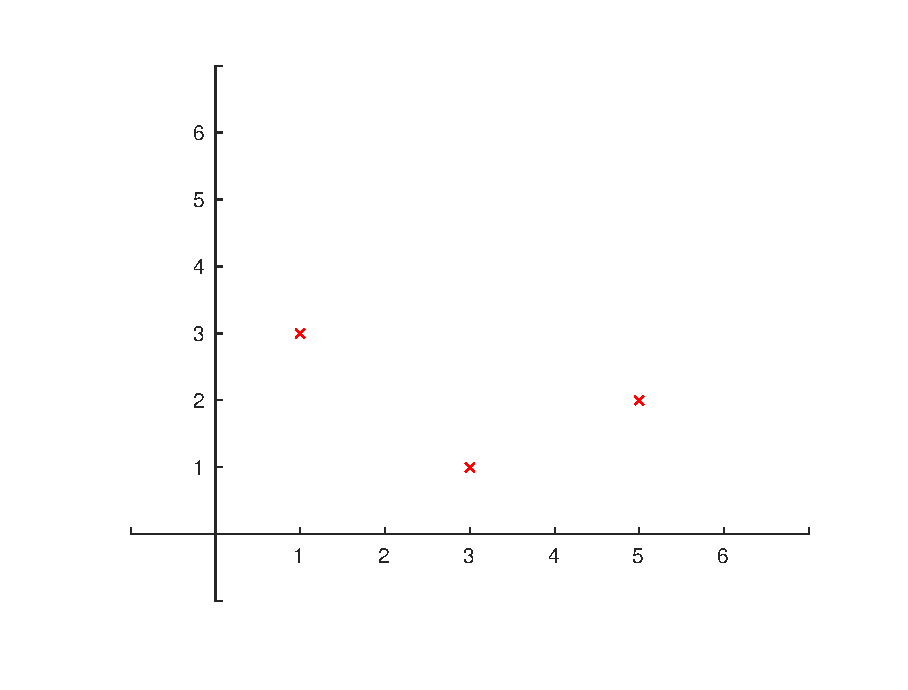
\includegraphics[width=\maxwidth{56.196688409433015em}]{figure_0}
\end{center}
\begin{par}
\begin{flushleft}
We see that there are only two planes in reality and they intersect in the line given by the reduced row echelon form matrix: $x+2y=-2;\;z=2$.
\end{flushleft}
\end{par}


\begin{par}
\begin{flushleft}
Now in this case, the third row is the sum of the first two rows.
\end{flushleft}
\end{par}

\begin{matlaboutput}
A = 3x4    
     1     2     2     2
     2     4     6     8
     3     6     8    10

\end{matlaboutput}
\begin{matlaboutput}
reduced_form = 3x4    
     1     2     0    -2
     0     0     1     2
     0     0     0     0

\end{matlaboutput}
\begin{center}
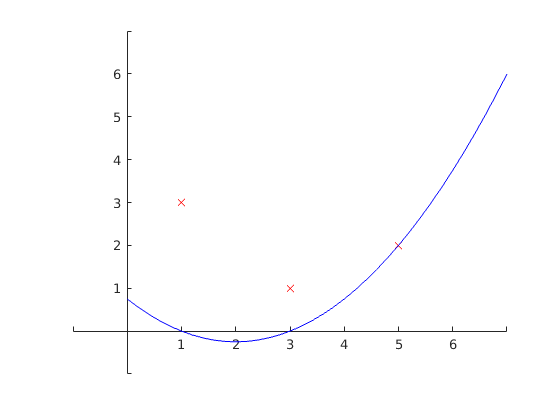
\includegraphics[width=\maxwidth{56.196688409433015em}]{figure_1}
\end{center}
\begin{par}
\begin{flushleft}
In this case we have three independent planes that, nevertheless, don't produce a unique solution because they all contain the same line. That's to say, the third plane contains the line of intersection of the first two planes and so doesn't constrict the result any further. This results in the solution space being a line.
\end{flushleft}
\end{par}


\begin{par}
\begin{flushleft}
Now we move the plane in the 3rd row by changing its component in the solution vector. Now there is no solution to this system as the plane in the 3rd row is parallel to the line of intersection of the other two planes but does not go through the line.
\end{flushleft}
\end{par}

\begin{matlaboutput}
A = 3x4    
     1     2     2     2
     2     4     6     8
     3     6     8   300

\end{matlaboutput}
\begin{matlaboutput}
reduced_form = 3x4    
     1     2     0     0
     0     0     1     0
     0     0     0     1

\end{matlaboutput}
\begin{center}
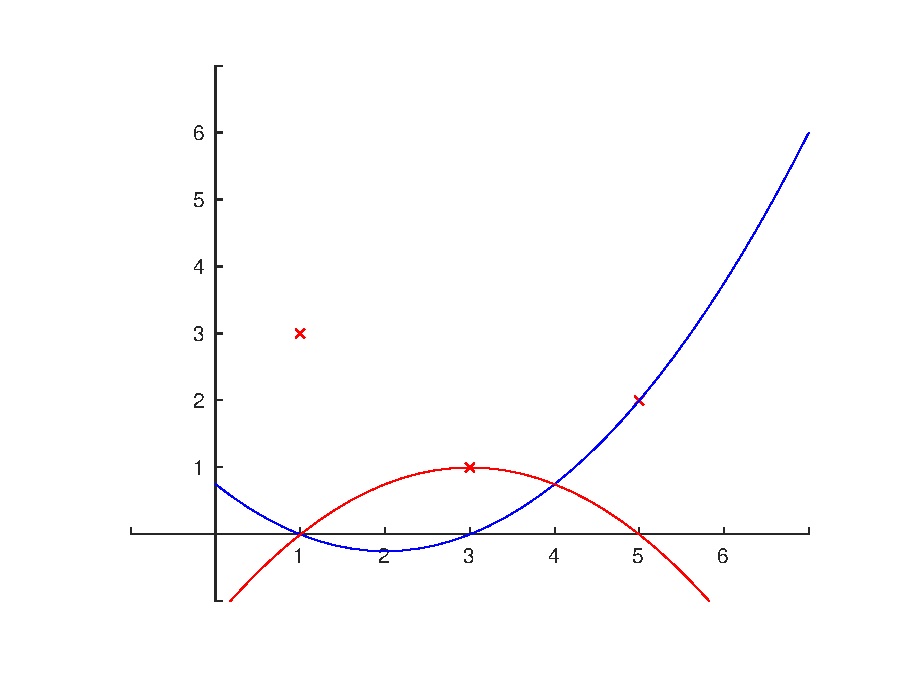
\includegraphics[width=\maxwidth{56.196688409433015em}]{figure_2}
\end{center}
\begin{par}
\begin{flushleft}
Looking at the matrix as a linear transformation from one co-ordinate space to another, consider \textbf{Ax} =\textbf{ y} where \textbf{x} is a column vector transformed by the matrix \textbf{A} into the vector \textbf{y}.
\end{flushleft}
\end{par}

\begin{matlaboutput}
A = 2x2    
     3     2
     1     4

\end{matlaboutput}
\begin{matlaboutput}
x = 2x4    
     0     1     1     0
     0     0     1     1

\end{matlaboutput}
\begin{par}
\begin{flushleft}
We transform the unit square in \textbf{x} using the matrix \textbf{A}.
\end{flushleft}
\end{par}

\begin{matlaboutput}
y = 2x4    
     0     3     5     2
     0     1     5     4

\end{matlaboutput}
\begin{center}
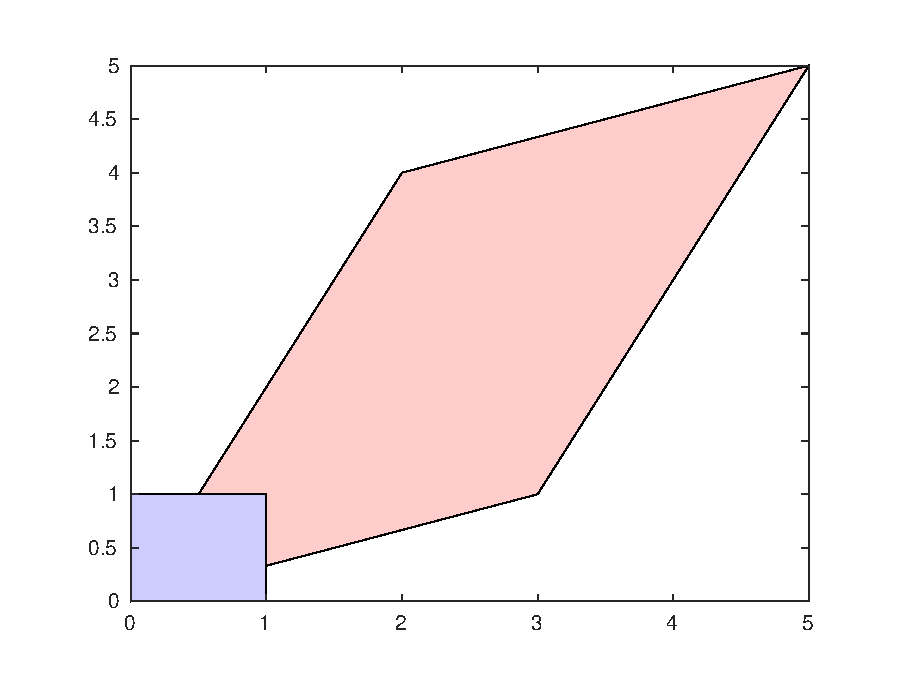
\includegraphics[width=\maxwidth{56.196688409433015em}]{figure_3}
\end{center}
\end{document}
